\documentclass[cover]{isas-seminar}

\usepackage{subfigure}
\usepackage{booktabs}

% Hier die Art der Veranstaltung eintragen (Seminar, Proseminar, Praktikum)
\eventtype{Praktikum} 
%\eventtype{Seminar} 
%\eventtype{Proseminar}
 
% Hier Titel der Veranstaltung eintragen 
\seminartitle{Forschungsprojekt Anthropomatik praktisch erfahren}
%\seminartitle{Modellbasierte Verfahren für intelligente Systeme}

\title{Projekt 2: Analyse von Schüttgutverhalten unter Verwendung von integrierter Sensorik}
\author{Andrea Bittner, Maren Kucza}

\begin{document}
\maketitle

\begin{abstract}
%Hier eine kommt die Zusammenfassung
\end{abstract}
\clearpage
\tableofcontents
\cleardoublepage

\section{Einleitung}

Das Projekt basiert auf der FlexSort-Anlage, eine optische Bandsortieranlage für Schüttgut am Fraunhofer IOSB. Die Sortieranlage kann Schüttgut mit Hilfe einer Flächenkamera optisch klassifizieren und mittels Druckluftdüsen voneinander trennen. Damit eine konstante und gleich verteilte Menge von Schüttgut auf dem Band liegt, wird mittels Rüttler das Material freigegeben und rutscht über eine Rutsche auf das Band. Die nachfolgenden Abbildungen \ref{fig:k1_flexsort1} bis \ref{fig:k1_flexsort3} zeigen den FlexSort.

\begin{figure}[htb]
	\centering
	\begin{minipage}[t]{0.4\linewidth}
		\centering
		\includegraphics[width=1\linewidth]{images/k1-flexsort1.jpg}
		\caption{FlexSort: Schüttgut fällt vom oberen Querrüttler auf den kurzen Rüttler und rutscht dann auf das Sortierband}
		\label{fig:k1_flexsort1}
	\end{minipage}% <- sonst wird hier ein Leerzeichen eingefügt
	\hfill
	\begin{minipage}[t]{0.54\linewidth}
		\centering
		\includegraphics[width=\linewidth]{images/k1-flexsort2.jpg}
		\caption{FlexSort: Sortierband mit optischer Objekterkennung und Druckluftdüsen zum Ausblasen}
		\label{fig:k1_flexsort2}
	\end{minipage}
\end{figure}

\begin{figure}[htb]
	\centering
	\includegraphics[width=0.5\linewidth]{images/k1-flexsort3.jpg}
	\caption{FlexSort: Außenansicht mit großem Rüttler und Förderbändern um Schüttgut für geschlossenen Messlauf wieder nach oben zu befördern}
	\label{fig:k1_flexsort3}
\end{figure}
 
Da die Klassifizierung und das Ausblasen von Teilchen etwas verzögert stattfinden, ist eine zeitlich gut geplante Aktivierung der Druckluftdüsen notwendig, um die Anlage möglichst kostensparend und effizient zu betreiben. Hierfür muss die genaue Position der auszusortierenden Teilchen zum Zeitpunkt der Düsenüberquerung ermittelt werden. Dabei ist zu beachten, dass sich das Schüttgut vom Klassifizierungszeitpunkt bis zum Zeitpunkt des Ausblasens auf dem Band bewegt. Die Bewegung der Teilchen kann unter Umständen von einzelnen Parametern der Anlage beeinflusst werden und wirkt sich dadurch auf das Sortierergebnis aus. Beispielsweise kann die Geschwindigkeit des Bandes dazu führen, dass die Teilchen darauf springen oder der Rüttler durch ungünstige Vibrationsbewegungen keine konstante Menge von Teilchen über die Rutsche auf das Band frei gibt. 

In diesem Projekt soll eine Möglichkeit gefunden werden, den Prozess des Sortierens von Schüttgut genauer zu verstehen und dadurch weitere Optimierungen an der Anlage und im Prozess vornehmen zu können. So könnte ein stabileres Sortierergebnis erreicht werden. Neben den rein optisch gewonnen Daten können weitere Messwerte durch andere Verfahren unterstützend sein. In diesem Projekt soll dies mit Hilfe eines instrumentierten Schüttguts passieren, über den Bewegungsdaten gesammelt und ausgewertet werden können. Es soll untersucht werden, ob sich in den gewonnen Daten bestimmte Bewegungsmuster erkennen lassen, die auf einzelne Anlagenmodule zurückgeführt werden können. Gegebenenfalls lassen sich zwischen den Anlagenmodulen verschiedene Korrelationen erkennen, die zukünftig zur Optimierung der Anlage genutzt werden können. Darüber hinaus könnte ein Qualitätsmaß erstellt werden, anhand dessen die gewählten Parameter der Anlage bewertet werden.

 %Projektbeschreibung
\section{Projektplanung}

\subsection{Aufgabenstellung}

Im Rahmen des Forschungspraktikums soll ein Schüttgut konstruiert werden, dass über Sensorik verfügt, mit der genauere Positions- und Lagedaten gemessen werden können. Das Schüttgut soll die annähernde Größe des zu sortierenden Schüttguts haben. Die maximale Größe ist jedoch durch die Kapsel eines Überraschungs-Eis limitiert, in der die Sensorik untergebracht werden soll. Zunächst muss solch ein instrumentiertes Schüttgut entworfen werden.
 
Nach der Recherche von geeigneten Bauteilen soll ein Prototyp des Sensorik-Schüttguts erstellt werden, mit dem Daten auf einer Bandsortieranlage gewonnen werden können.

Zur Datengewinnung muss das Schüttgut programmiert werden, sodass die gelieferten Daten der Sensoren an eine Analysesoftware auf einem  PC/Laptop übertragen werden können. In einem weiteren Schritt sollen die gewonnen Daten ausgewertet werden. Hierfür muss eine Anwendung entwickelt werden, mit der sich die gewonnen Daten verständlich darstellen und analysieren lassen.
%TODO Qualtitätsmaß, Aufgabe anpassen
Die Werte der Sensoren müssen anschließend kalibriert und in Korrelation mit der tatsächlichen Laufbahn des Teilchens auf der Anlage gebracht werden. Hier soll eine Qualitätsgröße gefunden werden, die die Auswirkungen von verschiedenen Konfigurationsparametern der Anlage auf die Bewegung der Teilchen beschreibt und bewertet. 
Abschließend soll validiert werden, ob mit Hilfe von instrumentierten Schüttguts ein verbessertes Ergebnis der Bandsortieranlage erzielt werden kann.

Folgende Punkte beschreiben Herausforderungen, die großen Einfluss auf den weiteren Projektverlauf haben könnten:
\begin{description}
	\item [Begrenzte Größe:] Die Größe der Sensorik bestimmt zum einen, auf welche Anlage anschließende Messungen durchgeführt werden können, da das instrumentiertes Schüttgut zur Größenordnung des zu sortierenden Schüttgutes passen muss. Zum Anderen wirkt sich dies stark auf die Wahl der verwendeten Bauteile aus, die im verbundenen Zustand Platz in der Kapsel eines Ü-Eis finden müssen
	\item [Implementierung:] Gesammelte Daten über Sensoren müssen an den PC weitergeleitet werden. Hierfür gibt es verschiedene Möglichkeiten (Daten loggen oder per Funk direkt übertragen).
	\item [Bewertung der Daten:] Die gelieferten Daten von den Sensoren müssen aufbereitet werden, bevor sie interpretiert werden können.
	\item [Korrelation gemessene Daten zu Anlageparametern:] Finden einer Korrelation, Definition eines Qualitätsmaßes; Evaluation der Methode, durch instrumentiertes Schüttgut weitere Daten für die Optimierung der Anlage zu gewinnen 
\end{description} 

\subsection{Zeitliche Planung}
Die beschriebenen Herausforderungen spiegeln sich auch in den Meilensteinen des Projektes wieder:
\begin{description}
	\item [Meilenstein 1] beinhaltet das Design eines Schüttguts mit Sensorik, das die maximale Größe eines Ü-Eis hat. Zusätzlich wurde eine Machbarkeitsstudie durchgeführt, mit der die Wahl der Bauteile begründet werden kann.
	\item [Meilenstein 2] beinhaltet die Fertigung und Programmierung des Schüttguts mit Sensorik. Nach Abschluss liegt ein fertiges und funktionsfähiges instrumentiertes Schüttgut vor, das gemessene Daten per Bluetooth überträgt.
	\item [Meilenstein 3] umfasst das Sammeln und Darstellen von Daten aus der Anlage mit Hilfe des instrumentierten Schüttguts. Nach ausreichender Anzahl von Testdaten und Aufbereitung sowie Darstellung in einem Verständlichen Format ist der Meilenstein erreicht.
	\item [Meilenstein 4] beinhaltet die Analyse der Daten und die Findung einer Korrelation zu den Parametern der Schüttgutanlage. Eine gefundene Qualitätsgröße wurde definiert.
	\item [Meilenstein 5] schließt das Projekt mit der Evaluation der Ergebnisse ab. Es liegt nach Projektende eine Bewertung für das Verfahren vor, in dem mit  weiteren gewonnen Daten (außer den optischen) der Sortierprozess positiv beeinflusst werden kann.
\end{description}
	
Um das neue Verfahren zur Datengewinnung zu evaluieren, sind folgende Arbeitsschritte geplant: \newpage

\begin{figure}[ht]
	\centering
	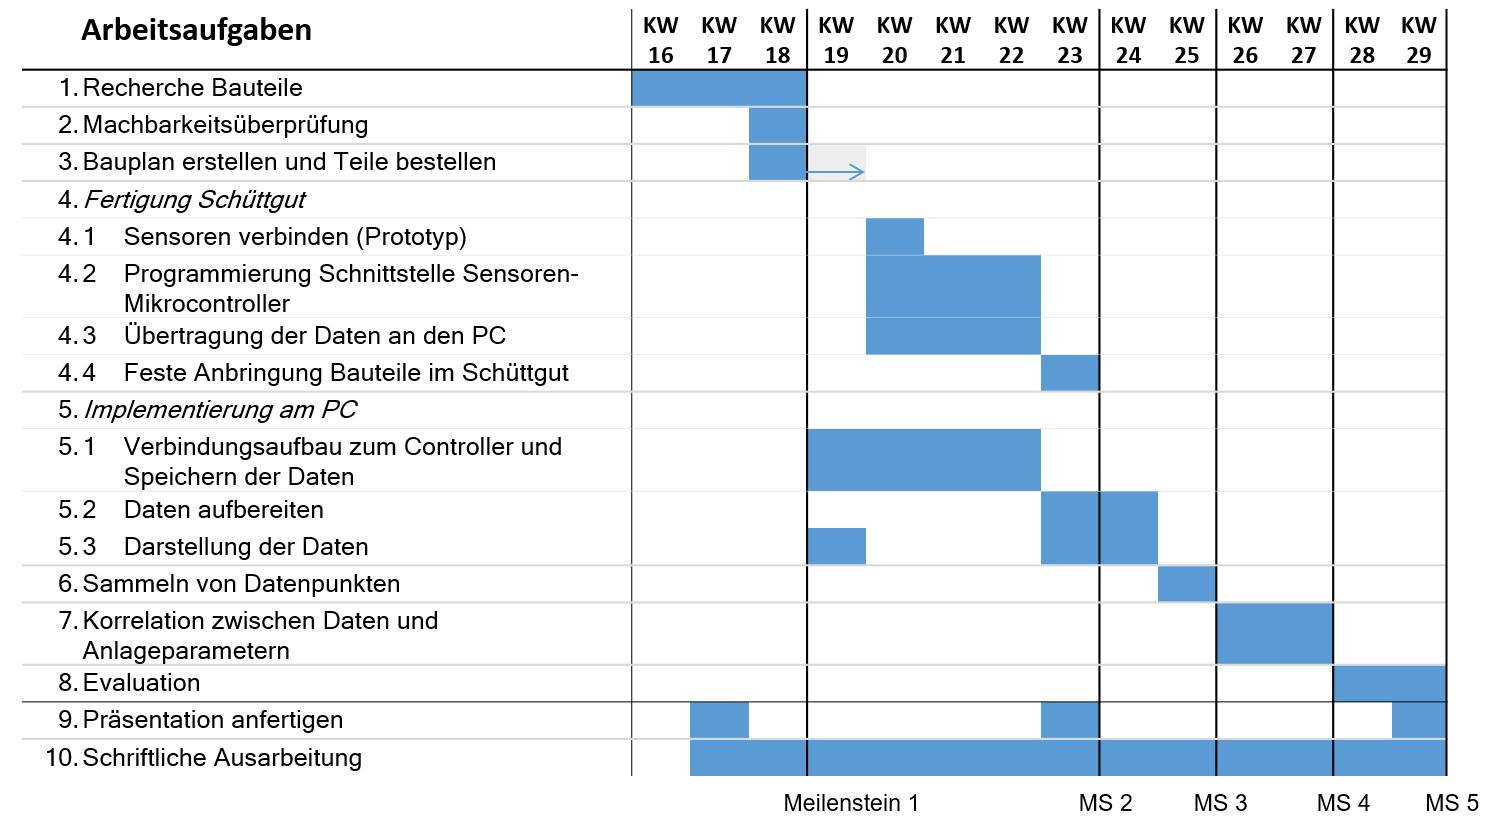
\includegraphics[width=1\textwidth]{images/k2-projektplan.JPG}
	\caption {Projektplanung runtergebrochen auf einzelne Arbeitsschritte}
	\label{fig:k2}
\end{figure}

Meilenstein 1 ist für die ersten drei Projektwochen angesetzt. Die grau markierte Kalenderwoche 19 bei Aufgabe 3 wird für die Bestelldauer der Bauteile geblockt. Solange kann nicht mit den Aufgabenteilen 4.* begonnen werden. Allerdings können einzelne Aufgaben aus Teil 5.* vorgezogen werden. Fortführend werden die Aufgaben 4 und 5 parallel bearbeitet, wobei Meilenstein 2 nach Kalenderwoche 23 ein fertiges instrumentiertes Schüttgut aufweist. Meilenstein 3 wird zwei Wochen später nach beenden von Aufgabenteil 5 und dem Sammeln von Testdaten erreicht. Ab Kalenderwoche 26 beginnt die Analyse der Daten für den Abschluss von Meilenstein 4. Die letzten beiden Wochen sind für die Evaluation des Projektes angesetzt, womit auch Meilenstein 5 erreicht wird. Zusätzlich sollte das Projekt fortlaufend dokumentiert sowie drei Präsentationen ausgearbeitet werden. %Projektplanung
\section{Projektdurchführung - noch überarbeiten}

\subsection{Design des instrumentierten Schüttguts}
Allgemeine Anforderungen an das instrumentierte Schüttgut:

\begin{itemize}
	\item Möglichst klein (die Mindestgröße wir durch die Größe des Mikrocontrollers und der Sensoren bestimmt)
	\item Aufnehmen von Bewegungsdaten
	\item Übertragung von Daten an einen PC
	\item Betrieben durch interne Batterie
	\item Optional: Cachen von Daten, bis diese ausgelesen werden 
\end{itemize}

\subsubsection*{Größe des instrumentierten Schüttguts}

Das instrumentierte Schüttgut soll in eine Kapsel eines Kinder Überraschungseis passen. Dadurch wird die maximale Größe des Schüttguts festgelegt. Die Wahl der Ü-Ei-Kapsel als Hülle für das Schüttgut eignet sich dahingehend gut, dass er einerseits den Mikrocontroller schützt, andererseits sehr einfach zu beschaffen ist und kein Behältnis aufwendig produziert werden muss (zum Beispiel als 3D-Druck).

Maße der Kapsel aus einem Kinder Überraschungsei
%TODO Bild

\subsubsection{Mikrocontroller}

Der Mikrocontroller ist die Hauptplatine, an der alle anderen Bauteile angeschlossen werden müssen. Ausschlaggebend für die Wahl des Mikrocontrollers ist vor allem die Größe des Bauteils. 

Gewähltes Bauteil: Adafruit Pro Trinket 3V 12MHz

Der Pro Trinket 3V 12MHz von Adafruit besitzt einen leistungsstarken ATmega328-Chip, der auch auf einigen Arduino-Mikrocontrollern verwendet werden. Er besitzt einen Speicher von 28K und einen RAM von 2K. Vorteile sind bei diesem, dass er jedoch mit 18 GPIOs (General Purpose Input Output) und 2 analogen Anschlüssen weitaus mehr Anschlussmöglichkeiten bietet, als beispielsweise der Arduino Pro Mini. Die Maße des Boards sind  38mm x 18mm x 4mm, sodass die Platine ausreichend Platz in der Kapsel haben sollte. Auf dem Trinket ist ein USB Bootloader vorinstalliert, sodass der Mikrocontroller per USB programmiert werden kann. (Quelle: https://www.adafruit.com/products/2010)


%So werden Bilder eingebunden (als pdf, jpg oder png)
%\begin{figure}[ht]
%  \centering
%  \caption{Hier kommen weitere Erklärungen zum Bild}
% \label{fig:autorname_bild1}
%\end{figure}
%
% Auf diese Abbildung wird dann mit Abb. \ref{fig:autorname_bild1} verwiesen. %Projektdurchführung
\section{Musterdoc aus Vorlage}

\subsection{Grundlagen des Filters XY}
Vektoren und Matrizen
%
\begin{equation*}
	\vec{x}, \mat{A}
\end{equation*}
%
Mengenzeichen
%
\begin{equation*}
	\IR, \IN
\end{equation*}
%
Zufallsvariablen, etc...
%
\begin{equation*}
	\rv{y}, \rvv{z},
	\Var, \E, \Cov
\end{equation*}
%
Bitte nur Gleichungen nummerieren, auf die sich auch später bezogen wird
%
\begin{equation}
	a = b +c \enspace .
	\label{eq:NameDergleichung}
\end{equation}
%
Laut (\ref{eq:NameDergleichung}) ist $a=b+c$.

Mehrzeiliger Formelsatz mit \emph{align}
%
\begin{align*}
	a &= b + c \enspace ,\\
	a_{ij} &= b_{ij} + c_{ij} \enspace .
\end{align*}
%
oder mit \emph{multline}
%
\begin{multline*}
	a_{2343443} = \\
	b + c + \frac{3464421}{32455767567567575677} 
	\cdot \left( b_{ij} + c_{ij} \right)
	\cdot \int_{x=55}^{88} x^{67823+x} \frac{x}{32455767567567575677} \text{d}x
	\enspace .
\end{multline*}
%

%So werden Bilder eingebunden (als pdf, jpg oder png)
%\begin{figure}[ht]
%  \centering
%  \caption{Hier kommen weitere Erklärungen zum Bild}
% \label{fig:autorname_bild1}
%\end{figure}
%
% Auf diese Abbildung wird dann mit Abb. \ref{fig:autorname_bild1} verwiesen.

\bibliographystyle{plain}
\begin{thebibliography}{99}
	
	\bibitem{bib:russel_norvig} {\sc S. Russel and P. Norvig }  \textit{Artificial Intelligence - A Modern Approach},
	Second Edition, Prentice Hall, 2003.
	
\end{thebibliography}



\end{document}
